\documentclass[11pt]{article}


\usepackage[a4paper,top=1.5cm,bottom=2cm,left=1.5cm,right=1.5cm,marginparwidth=0cm]{geometry}
\usepackage[T1]{fontenc} % codifica dei font
\usepackage[utf8]{inputenc} % lettere accentate da tastiera
\usepackage[italian]{babel} % lingua del documento
\usepackage{url} 
\usepackage{quoting}
\usepackage{xspace}% per lo spazio intelligente
\usepackage{titlesec} % per formato custom dei titoli dei capitoli
\usepackage{tcolorbox}%per i box

\usepackage{amsmath}
\usepackage{graphicx}
%\usepackage[colorlinks=true, allcolors=blue]{hyperref}
\usepackage{mathrsfs}
\usepackage{caption}
\usepackage{hyperref}
\hypersetup{
    colorlinks=false,
    linkcolor=blue,
    filecolor=magenta,      
    urlcolor=cyan,
    pdftitle={ProgrammazioneAvanzata-c++},
    pdfpagemode=FullScreen,
    }
\urlstyle{same}

\usepackage{afterpage}

\newcommand\blankpage{%
    \null
    \thispagestyle{empty}%
    \addtocounter{page}{-1}%
    \newpage}
    
\usepackage{circuitikz}
\usepackage{multirow}

\usepackage{listings}
\usepackage{xcolor}

\definecolor{codegreen}{rgb}{0,0.6,0}
\definecolor{codegray}{rgb}{0.5,0.5,0.5}
\definecolor{codepurple}{rgb}{0.58,0,0.82}
\definecolor{backcolour}{rgb}{0.95,0.95,0.92}

\lstdefinestyle{mystyle}{
    backgroundcolor=\color{backcolour},   
    commentstyle=\color{codegreen},
    keywordstyle=\color{magenta},
    numberstyle=\tiny\color{codegray},
    stringstyle=\color{codepurple},
    basicstyle=\ttfamily\footnotesize,
    breakatwhitespace=false,         
    breaklines=true,                 
    captionpos=b,                    
    keepspaces=true,                 
    numbers=left,                    
    numbersep=5pt,                  
    showspaces=false,                
    showstringspaces=false,
    showtabs=false,                  
    tabsize=2
}

\lstset{style=mystyle}

\begin{document}

\pagestyle{plain}

\thispagestyle{empty}

\begin{center}

  \begin{figure}[h!]
  \centering
    
\includegraphics[trim= 1cm 3.5cm 8.1cm 24.2cm, clip]{img/unitnlogo.pdf}
  \end{figure}

  \vspace{2 cm} 

  \LARGE{Dipartimento di Ingegneria e Scienza dell’Informazione\\}

  \vspace{1 cm} 
  \Large{Corso di Laurea in\\
    %Informatica
    Ingegneria Informatica, delle Comunicazioni ed Elettronica
    %Ingegneria dell'Informazione e Organizzazione d'Impresa
    %Ingegneria Elettronica e delle Telecomunicazioni
  }

  \vspace{2 cm} 
  %\Large\textsc{Manuale di Fisica I\\} 
  %\vspace{1 cm} 
  \Huge\textsc{Corso di Programmazione Avanzata\\}
   \vspace{1 cm} 
  \Large{\it{Linguaggio C++ 11}}


  \vspace{2 cm} 
  % \begin{tabular*}{\textwidth}{ c @{\extracolsep{\fill}} c }
  % \Large{Docente} & \Large{Studenti}\\
  % \Large{Luca Matteo Martini}& \Large{Cristiano Berardo}\\
  % &\Large{Davide Scarano}\\
  % &\Large{Raffaele Cella}
  % \end{tabular*}

  \vspace{2 cm} 

  \Large{Anno accademico 2023/2024}

\end{center}
\blankpage

\section{UML}

\section{Ridefinizione degli operatori}
Il linguaggio C++ supporta la ridefinizione degli operatori. Gli operatori sono le operazioni che appaiono nelle espressioni.

Supponiamo di avere A a1,a2, a3, a4; nell’espressione
a1=(a2+a3)*(++a4); compaiono quattro operatori operator=,
operator+, operator* e operator++.
operator++ ha un solo operando mentre operator=, operator+,
operator* ne hanno due. 

\paragraph{}
Gran parte degli operatori si possono ridefinire o come metodi
della classe o come funzioni esterne, ma NON le due cose
assieme.
Quando si ridefiniscono come metodi il primo operando
corrisponde all’istanza chiamante e gli altri (se ve ne sono) a
parametri del metodo.
Quando si ridefiniscono come funzioni esterne alla classe TUTTI
gli operandi corrispondono a parametri della funzione. 
\paragraph{}
operator= si puo’ ridefinire SOLO come metodo ovvero

\begin{lstlisting}[language=c++]
    A& A::operator=(const A&)
\end{lstlisting}


\subsection{Ridefinizione operator<<}

\begin{lstlisting}[language=c++]
    class A{
        ...

        friend ostream& operator<<(ostream &os, const A& _a);
    }
    ostream& operator<<(ostream &os, const A& _a);
\end{lstlisting}

\subsection{Ridefinizione operator+}
\begin{lstlisting}[language=c++]
    class A{
        ...
        A operator+(const A&); 

        //modo da preferire
        friend A operator+(const A&,const A&);
    }
    A operator+(const A& _x, const A& _y);
\end{lstlisting}
\subsection{Ridefinizione operator-}

\begin{lstlisting}[language=c++]
    class A{
        ...
        friend A operator-(const A& _c1, const A& _c2); 
    }
    A operator-(const A& _c1, const A& _c2); 
\end{lstlisting}
\subsection{Ridefinizione operator*}
\begin{lstlisting}[language=c++]
    class A{
        ...
        friend A operator*(const A& _c1, const A& _c2);
    }
    A operator*(const A& _c1, const A& _c2); 
\end{lstlisting}
\subsection{Ridefinizione operator++}

\begin{lstlisting}[language=c++]
    class A{
        ...
        A& A::operator++();     //prefisso
        A A::operator++(int);   //postfisso
    }
\end{lstlisting}

\subsection{Distinzione sul tipo di ritorno}
Ci sono operatori che ritornano il risultato per valore e
operatori che ritornano il risultato per referenza. Come nel caso degli incrementi o decrementi prefissi o postfissi la distinzione si ha quando il risultato è utilizzato successivamente nella stessa espressione. 
\paragraph{}
Gli operatori che modificano l’oggetto chiamante
ritornando una reference. Esempio: operator+= e
operator+ il primo ritornerà A\& mentre il secondo A.


\subsection{Parola chiave friend}
Quando dentro una classe compare questa parola chiave la
riga NON e’ una dichiarazione di funzione o metodo ma piu’
semplicemente permette l’accesso alle parti private da parte di
una funzione o anche classe definita altrove. 

\section{Ereditarieta’}
In C++ vi sono tre tipi di ereditarieta’:

\begin{itemize}
    \item public
    \item private
    \item protected
\end{itemize}
Queste sono anche le stesse keywords della visibilita’ nella classe.

\begin{table}[ht]
\caption{Ereditarietà}
\begin{center}
\begin{tabular}{c|c|c}
    Tipo di Ereditarietà &Casse base& Casse derivata\\
    \hline
    \multirow{3}{*}{Public}     &Public&Public\\
                                &Protected&Protected\\
                                &Private&Inacc.\\
    \hline

    \multirow{3}{*}{Protected}     &Public&Protected\\
                                &Protected&Protected\\
                                &Private&Inacc.\\
    \hline
    \multirow{3}{*}{Private}     &Public&Private\\
                                &Protected&Private\\
                                &Private&Inacc.\\
    \hline
\end{tabular}
\end{center}
\label{tab:multicol}
\end{table}

\subsection{Keyword virtual}
I metodi possono essere definiti virtual, in questo modo C++ riesce a dichiara il late binding (risolto run-time) rispetto al early binding (risolto a compilation-time).
\paragraph{}
Una classe è detta \verb|Puramente virtuale| se ha almeno un metodo virtual, ovvero la sua dichiarazione nella classe è seguita da "=0":

\begin{lstlisting}[language=c++]
class A{ 
    virtual int metodo()=0;
    ...
};
\end{lstlisting}

Una classe puramente virtuale NON si può istanziare.
\section{Programmazione generica}
Si intende la possibilita’ data da un linguaggio di
rappresentare tipi e implementare algoritmi che
abbiano un tipo come parametro.
Il tipo parametrico viene poi specificato:
\begin{itemize}
    \item Tempo di compilazione (es. templates in C++)
    \item Tempo di esecuzione (es generics in Java)
\end{itemize}

Lo scopo è implementare algoritmi che siano
indipendenti dal tipo su cui operano.Idealmente al massimo livello di astrazione possibile.

\begin{lstlisting}[language=c++]
#include<string>
#include<utility>
#include<iostream>
using namespace std;

template <class T>
void my_swap(T& f, T& s) {
    T tmp = f;
    f = s;
    s = tmp;
}
int main(){
    int a = 3; int b = 4;
    my_swap<int> (a,b);     //a=4   b=3
    string s1 = "hello";
    string s2 = "world";
    my_swap<string> (s1,s2);  //s1=world   s2=hello
return 0;
}
\end{lstlisting}

\subsection{Utilizzo metodo clone:}
\begin{lstlisting}[language=c++]
class A{
    public:
    virtual A& operator=(const A& _a)=0;
    virtual A* clone()const=0;
    virtual ~A(){};
};
----
#include "A.h"
class B:public A{
    int i;
    public:
    B(int _i){i=_i;};
    B& operator=(const A& _b);
    B& operator=(const B& _b);
    B* clone()const;
    friend ostream& operator<<(ostream& os,const B& _b);
};
ostream& operator<<(ostream& os,const B& _b); 
----
#include "B.h"
B& B::operator=(const A& _b){
    A* temp=_b.clone();
    B b(*((B*)temp));
    *this=b;
    return *this;
}
B& B::operator=(const B& _b){
    i=_b.i;
    return *this;
}
B* B::clone()const{ return new B(*this);};
ostream& operator<<(ostream& os,const B& _b){return os<<_b.i;}

----

#include<string>
#include<utility>
#include<iostream>
using namespace std;
#include "B.h"

void my_swap (A &f, A &s ) {
    A* temp=f.clone();
    f=s;
    s=*temp;
    delete temp;
}
int main() {
    B x(33);
    B y(44);
    cout << x << y << endl;
    my_swap(x,y);
    cout << x << y << endl;
    return 0;
}
\end{lstlisting}
\section{Standard Template Library}

La Standard Template Library (STL) è una libreria software per il linguaggio di programmazione C++ che definisce quattro componenti principali: contenitori, iteratori, algoritmi e funtori.
\paragraph{I contenitori } si dividono in sequenziali e associativi:

\begin{itemize}
    \item[--] I contenitori standard sequenziali includono \verb|vector|, \verb|list|e \verb|deque|;
    \item[--] I contenitori standard associativi sono invece: \verb|set|, \verb|multiset|,  \verb|map |e \verb|multimap |.
\end{itemize}

\begin{table}[h]
    \centering
    \begin{tabular}{c|c}
    \hline
            Contenitore&Descrizione\\
    \hline
         \verb|vector|  &  Array dinamico capace di ridimensionarsi, elementi contigui\\
                        & accesso, inserimento e cancellazione in coda \textbf{O(1)}\\
                        & inserimento in testa, ricerca, cancellazione \textbf{O(n)} \\
    \hline
         \verb|list|    & lista bidirezionale, elementi non contigui in memoria \\                         
                        & accesso e ricerca mediante \textit{iteratore} \textbf{O(n)} \\
                        & inserimento e cancellazione  contigui\\
    \hline\hline
         \verb|set| & insieme ordinato (piccolo-grande) senza duplicati, elementi non contigui\\
                    & il valore degli elementi non può essere modificato\\
                    & ricerca, inserimento e cancellazione \textbf{O(log(n))}\\
                    &implementazione BST\\
                    &\verb|unordered_set| nessun ordinamento, no duplicati in media \textbf{O(log(1))}\\
                    &implementazione hash table\\
                    \hline
         \verb|multiset|& uguale al set ma consente duplicati\\
                        &\verb|unordered_multiset| uguale al unordered\_set ma con duplicati \\
                    \hline
         \verb|map| & array associativo <key, value> ordinato rispetto alla chiave \\
                    & generalmente \textbf{O(log(n))}\\
                    &\textbf{O(log(1))} se si accede tramite operator[]\\
                    &\verb|unordered_map| non ordinato, \textbf{O(log(1))} \\
                    \hline
         \verb|multimap|& come map, ma può contenere più valori uguali \\
                
    \end{tabular}
    \caption{Contenitori STL}
    \label{tab:my_label}
\end{table}


\section{Iteratori}
Oggetto che consente di visitare tutti gli elementi contenuti in un altro oggetto, tipicamente un contenitore, senza doversi preoccupare dei dettagli di una specifica implementazione. Un iteratore è talvolta chiamato cursore, specialmente nel contesto delle basi dati.

\begin{lstlisting}[language=c++]
#include <iostream>
using namespace std;
#include<list>
int main(int argc, char *argv[]){
    list<int> l;
    l.push_back(2);
    l.push_front(3);
    list<int>::iterator it; //c++98
    for(it=l.begin();it!=l.end();++it)
        cout<<*it;
    for(auto a=l.begin();a!=l.end();++a) //c++11 e successivi
        cout<<*a;
    for(auto& e:l)
        e++;                //out: 43
    cout<<l.front() << l.back();    //out: 43
    l.push_back(2);
    l.push_front(5);
    l.pop_back();
    l.pop_front(); 

    auto a=l.cbegin();//const_iterator  l=74
    l.push_front(8);l.push_front(9);    //l=9874
    cout<<endl<<*a;     //7

    list<int> l2;
    l2.splice(l2.cbegin(),l,a,l.cend());    //l: 98 and l2: 74
    l2.swap(l);                             //l: 74 and l2: 98

    cout<<l.size();     //2
    
    l.reverse();    //47
    l.sort();       //47 (773344->334477)
    l.unique();     //47 (347)
    l2.sort()       //89
    l.merge(l2);    //l: 4789 l2: 

    //--reverse iterator--

    list<int>::reverse_iterator rit;
    for(rit=l.rbegin();rit!=l.rend();++rit)
        cout<<*rit;                            //9874
    for(auto a=l.rbegin();a!=l.rend();++a)
        cout<<*a;

    l.resize(3);            //l: 478
    l.remove(7);            //l: 48
    l.erase(l.begin());     //l: 8
    a=l.emplace(l.cbegin(),11); //l: 118
    l.push_front(13)            //l: 13118

    l2.assign(a,l.cend());      //l: 13118 l: 118

    list<int> l3(l);        //l3: 13118
    l=l2;                   //l: 118    l2:118

    l.clear();              //l: 
    cout<<endl<<l.max_size();   //768614336404564650
}
    
\end{lstlisting}


\section{set \& map}
Sono ordinati e usano operator<, non hanno il concetto di front e back, ma si usa \verb|insert|. Per utilizzare l'inserimento in map si deve utilizzare un nuovo operatore \verb|pair<T,T>|

\begin{lstlisting}[language=c++]
#include <iostream>
using namespace std;
#include<set>
#include<map>

int main(int argc, char *argv[]){
    set<A> s;
    s.insert(A()); // funziona solo se definito A::operator<
    map<A,int> m;
    m.insert(pair<A,int> (A(),2));// funziona solo se definito A::operator<
    map<int,A> ma;
    ma.insert(pair<int,A> (3,A()));//funziona,operator< definito per int
    ma[3]=A(); //equivalentemente per il map e' ridefinito operator[]            
}    
\end{lstlisting}


\section{multiset \& multimap}
Sono simili ai loro genitori: permettono di avere più elementi con lo stesso valore. Non può essere usato \verb|operator[]|.
\section{STL <algorithm>}
Alcune funzioni della libreria algorithm, per l'elenco completo si veda il seguente \href{https://cplusplus.com/reference/algorithm/}{link}

\begin{itemize}
    \item \verb|all_of|: Test condition on all elements in range
    \item \verb|any_of|:	Test if any element in range fulfills condition
    \item \verb|none_of|:	Test if no elements fulfill condition
    \item \verb|for_each|:	Apply function to range
    \item \verb|find|:	Find value in range
    \item \verb|find_if|:	Find element in range
    \item \verb|find_if_not|:	Find element in range (negative condition)
    \item \verb|count_if|:	Return number of elements in range satisfying condition
    \item \verb|mismatch|:	Return first position where two ranges differ
    \item \verb|equal|:	Test whether the elements in two ranges are equal
    \item \verb|is_permutation|:	Test whether range is permutation of another
    \item \verb|copy|:	Copy range of elements
    \item \verb|replace|:	Replace value in range (function template)
    \item \verb|replace\_if|:	Replace values in range
    \item \verb|remove|:	Remove value from range
    \item \verb|random_shuffle|:	Randomly rearrange elements in range
    \item \verb|reverse|:	Reverse range
    \item \verb|rotate|:	Rotate left the elements in range
    \item \verb|sort|:	Sort elements in range
\end{itemize}
\section{Puntatori e Funzioni}
Variabili che contengono indirizzi a funzioni. Questi servono quando il programma deve scegliere quale funzione chiamare fra diverse possibili, e la scelta non è definita a priori ma dipende dai dati del programma stesso.

Questo processo si chiama late binding: gli indirizzi delle funzioni da chiamare non vengono risolti al momento della compilazione, come avviene normalmente (early binding) ma al momento dell'esecuzione.

\begin{lstlisting}[language=c++]
    int a(double,int){...}
    int b(double,int){...}
    int f(int i,int j){return i*j;}
    int f2(int i, int j){return i+j;}
    double media_generale(int i, int j,int(*pf)(int,int) ){ 
        return double(pf(i,j))/2; 
    }
    main(){
        int (*pf)(int,int);
        int (*pfunz)(double, int);        
        ...
        if(i%2==0){
            pfunz=a;
        }else
            pfunz=b; 
        }   
        cout<<pfunz(2.0,3); //or cout<<(*pfunz)(2.0,3);

        pf=f;
        cout<<pf(2,3)<<endl; // or (*pf)(2,3);  //6
        cout<<media_generale(2,3,f)<<endl;      //3
        cout<<media_generale(2,3,f2)<<endl;     //2.5
    }
\end{lstlisting}

\section{Eccezioni}
Gli errori di runtime sono quegli errori che NON possono essere
rilevati in fase di compilazione, perché si manifestano solo durante
la fase di esecuzione del programma e solo in alcune particolari
circostanze, ossia ai veri casi di “eventi eccezionali”.
\paragraph{}
Alcuni esempi:

\begin{itemize}
    \item[--] divisione per 0;
    \item[--] pathname non valido o che fa riferimento ad una periferica che in un certo momento risulta scollegata;
    \item[--] overflow su un tipo di dato
    \item[--] operazione di casting non valido
\end{itemize}

Si tratta di errori pericolosi perché se non gestiti, possono generare
anomalie di funzionamento che possono determinare persino il
blocco inaspettato del programma.

Un’eccezione non necessariamente deve essere gestita all’interno
della stessa funzione in cui viene sollevata. Questo è reso possibile dal meccanismo proprio delle eccezioni, il
quale prevede che un’eccezione sollevata in una funzione e che non
venga in essa gestita, sia propagata all’indietro verso il chiamante,
si dice risalendo lo stack delle chiamate.


\subsection{throw}
Per gestire questi errori i linguaggi OOP implementano il meccanismo delle eccezioni, il quale consente di sollevare, \verb|throw|, un'eccezione quando si verifica un errore a runtime. Questo meccanismo si traduce nella creazione di un oggetto appartiene ad una classe particolare, dipendente dallo
specifico errore di runtime che si è verificato.

\subsection{try-cath}
Per "intercettare" l'errore in C++ viene fornito il costrutto \verb|try-cath| il quale permette di sospendere il programma nel punto dove si è verificato l'errore per saltare al pezzo di codice che gestisce l'errore.

\begin{lstlisting}[language=c++]
try{
    int x, y;
    //insert from keyboard
    if(y == 0) throw "Division by zero!";   //or division(x,y);
}catch(const char* msg){
    cerr<<msg<< endl;
}catch(){ }
...
\end{lstlisting}

\verb|try|:  blocco in cui si possono inserire le istruzioni che si vuole tenere “sotto controllo” perché durante l’esecuzione potrebbero generare degli errori a runtime.

\verb|catch|: blocco in grado di riconoscere e “catturare” un certo tipo di eccezione e che contiene le istruzioni per gestire l’errore di runtime che l’ha generata.
\paragraph{}
Quando nel blocco \verb|try| si genera un'eccezione si salta ai sui blocchi catch associati, partendo dal primo a scendere (dall'eccezione più specifica a quella più generale). Alla sua uscita il flusso del programma prosegue oltre l’ultimo blocco catch.


\subsection{stdexcept}
Questo header definisce un insieme di eccezioni standard che sia la libreria che i programmi possono utilizzare per segnalare errori comuni.
Includere nell'intestazione:\verb|#include <stdexcept>|.

\begin{itemize}
    \item Logic errors 
        \begin{itemize}
            \item \verb|logic_error|
            \item \verb|domain_error|
            \item \verb|invalid_argument|
            \item \verb|length_error|
            \item \verb|out_of_range|            
        \end{itemize}

    \item Runtime errors
        \begin{itemize}
            \item \verb|runtime_error|
            \item \verb|range_error|
            \item \verb|overflow_error|
            \item \verb|underflow_error|            
        \end{itemize}
\end{itemize}


\begin{lstlisting}[language=c++]
#include <stdexcept>
using namespace std;

int divideINT(int a, int b) {
    if (a < 0 || b < 0) {
        throw invalid_argument( "received negative value" );
    }
    return a/b;
}
void test(){
    int x=1, y=0; 
    try {
        cout << a << "/" << b << "=" << divideINT(a, b) << endl;
    } catch( const invalid_argument& e ) {
        cout << e.what(); << endl //or cout << "a or b negative" << endl;    //cout << e << endl; //bind ERROR    
    } cathc(...){   //otherwise
        cout << "other wrong error";
    }
}
int main(){ test(); }
\end{lstlisting}

\section{Multithreading in C++}
Dal C++ 11 si ha la casse \verb|thread|, la quale abilita alla scrittura di programmi che possono eseguire parti del codice in parallelo e non più in maniera sequenziale.

La classe \verb|thread| ha le seguenti funzioni:
\begin{itemize}
    \item detach
    \item get\_id
    \item join
    \item joinable
    \item join
    \item joinable
    \item native\_handle
    \item operator= (move semantics)
    \item hardware\_concurrency()
\end{itemize}


\begin{lstlisting}[language=c++]
#include <iostream>
#include <thread> 
using namespace std;

int a(){  /*do something...*/ }
int b(int count){ /*do something...*/ }

int main(){
    unsigned int c = thread::hardware_concurrency();
    thread t1 (a);
    thread t2;
    t2 = thread(b,0);

    t1.join();
    t2.join();
}
   
\end{lstlisting}

\subsection{Data race}
Si verifica quando due o più threads in un singolo processo accedono simultaneamente alla stessa area di memoria, almeno un accesso è eseguito in scrittura e non vi sono blocchi per l'accesso esclusivo. Questo significa che il valore da un momeno all'altro può essere cambiato ed alterare il funzionamento del programma.

Proprio per questo motivo in C++ vengono introdotti due blocchi: \verb|atomic| e \verb|mutex|.

\begin{itemize}
    \item \verb|atomic| rende atomiche le operazioni su una certa variabile;
    \item \verb|mutex| Definisco delle sezioni critiche come mutuamente esclusive nel codice;
\end{itemize}

\begin{lstlisting}[language=c++]
//first resolution with atomic 
#include <iostream>   
#include <thread>
#include <atomic>
using namespace std;

static std::atomic<int> count(0);
//static int count=0;
void inc_thread(){
    for(int i=0;i<10000;i++) count++;
}
void dec_thread(){
for (int i=0;i<10000;i++) count--;
}
main(){
    std::thread inc(inc_thread);
    std::thread dec(dec_thread);
    inc.join();
    dec.join();
    std::cout<<"counter"<<count;
    return 0;
} 
\end{lstlisting}

\begin{lstlisting}[language=c++]
//second resolution with mutex 
#include <iostream> 
#include <thread>
#include <mutex>
using namespace std;

mutex myMutex;
static int condivisa=0;
void inc_thread(){
    for(int i=0;i<10000;i++){
    myMutex.lock(); condivisa++; myMutex.unlock();}
}
void dec_thread(){
    for (int i=0;i<10000;i++){
    myMutex.lock(); condivisa--; myMutex.unlock();}
}
int main (){
    std::thread inc(inc_thread);
    std::thread dec(dec_thread);
    inc.join();
    dec.join();
}
\end{lstlisting}


\subsection{Problemi della concorrenza: deadlock e starvation}

\paragraph{Deadlock}
Situazioni in cui uno o piu’ processi/thread si bloccano:
\begin{itemize}
    \item Omettere l’unlock un mutex
    \item Terminazione inattesa di una funzione (lancio di eccezioni), soluzione: \verb|lock_guard<mutex>|
    \item Funzioni annidate che chiamano lo stesso mutex, soluzione: \verb|recursive_mutex|
    \item Ordine di locking di diversi mutex , soluzione: \verb|ock(mutex, mutex)|
\end{itemize}

\paragraph{Starvation} 
La politica di accesso impedisce ad un processo di accedere alla risorsa

\paragraph{}
Esistono nella letteratura altre primitive usando per
gestire la concorrenza come semafori e monitor ma non sono forniti dallo standard di C++ che
preferisce fornire primitive di livello più basso.
\section{Riferimenti: lvalues \& rvalues}

Un riferimento, analogamente a un puntatore, archivia l'indirizzo di un oggetto che si trova in un'altra posizione in memoria. A differenza di un puntatore, dopo l'inizializzazione non è possibile impostare un riferimento in modo che indichi un oggetto diverso o che sia impostato su Null. 
Esistono due tipi di riferimenti e operatori:
\begin{itemize}
    \item L'operatore \verb|&| indica: riferimenti \verb|lvalue| che fanno riferimento a una variabile denominata
    \item L'operatore \verb|&&| indica: riferimenti \verb|rvalue|, o un riferimento universale (\verb|rvalue| o \verb|lvalue|) a seconda del contesto,  che fanno riferimento a un oggetto temporaneo.
\end{itemize}

\begin{lstlisting}[language=C++]
#include <iostream>
using namespace std;

int main(){
    Person myFriend;    //struct with char* Name and Short Age
   
    Person& rFriend = myFriend;

    myFriend.Name = "Bill";
    rFriend.Age = 40;

    cout << rFriend.Name << " is " << myFriend.Age << endl; //Bill is 40
}
\end{lstlisting}

\subsection{lvalues: \&}
È possibile considerare un riferimento lvalue come nome alternativo per un oggetto.
Un riferimento deve essere inizializzato e non può essere modificato.


\subsection{Rvalue: \&\&}
I riferimenti Rvalue supportano l'implementazione della semantica di spostamento, che può aumentare significativamente le prestazioni delle applicazioni. La semantica di spostamento, \verb|move()|, consente di scrivere codice per il trasferimento delle risorse (ad esempio memoria allocata in modo dinamico) da un oggetto a un altro.
L’idea è che la proprietà di dati allocati nella memoria dinamica venga trasferita senza dover essere copiata. Lo scopo è aumentare l’efficienza del programma copiando meno dati possibili.

Per implementare la move semantics si fornisce:
\begin{itemize}
    \item costruttore di spostamento
    \item operatore di assegnazione di spostamento \verb|operator=| alla classe
    \item distruttore
\end{itemize}

\begin{lstlisting}[language=C++]
#include <iostream>
using namespace std;

int main(){
    int& x=6; //non compila
    const int& x=6; //compila
    //Dal c++11
    int&& i=7; // rvalue reference, Permette di fare riferimento ad un rvalue e di modificarlo
}
\end{lstlisting}
le reference usuali \verb|int \&| sono lvalue references.

Per comprendere meglio la semantica di spostamento, si consideri l'esempio dell'inserimento di un elemento in un oggetto \verb|vector|. Se viene superata la capacità dell'oggetto, l'oggetto \verb|vector| deve riallocare memoria sufficiente per i relativi elementi e quindi copiare ogni elemento in un'altra posizione di memoria per liberare spazio per l'elemento inserito. Quando un'operazione di inserimento copia un elemento, crea prima di tutto un nuovo elemento. Chiama quindi il costruttore di copia per copiare i dati dall'elemento precedente al nuovo elemento. Infine, elimina definitivamente l'elemento precedente. La semantica di spostamento consente di spostare gli oggetti direttamente senza dover eseguire operazioni di allocazione di memoria e copia costose.


\subsection{Value Categories}

\begin{itemize}
    \item \verb|glvalue|, general lvalue espressione la cui valutazione determina l'identità di un oggetto, di un campo di bit o di una funzione.
    \item \verb|prvalue|, pure rvalue espressione la cui valutazione inizializza un oggetto o un campo di bit oppure calcola il valore dell'operando di un operatore
    \item \verb|xvalue|, eXpiring value glvalue che denota un oggetto o un campo di bit le cui risorse possono essere riutilizzate, in genere perchè vicino a fine vita
    \item \verb|lvalue| è un glvalue che non è un valore xvalue.
    \item \verb|glvalue| è un prvalue o un valore xvalue.
\end{itemize}

\begin{figure}[h]
    \centering
    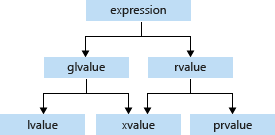
\includegraphics[width=0.4 \textwidth]{img/value.png}
    \caption{Value CategoriesValue}
\end{figure}

Un lvalue ha un indirizzo a cui il programma può accedere, ad esempio nomi di variabili.

Un'espressione prvalue non ha un indirizzo accessibile dal programma. Esempi di espressioni prvalue includono valori letterali, chiamate di funzione che restituiscono un tipo non di riferimento e oggetti temporanei creati durante la valutazione dell'espressione, ma accessibili solo dal compilatore.

Un'espressione xvalue ha un indirizzo che non è più accessibile dal programma, ma può essere usato per inizializzare un riferimento rvalue, che fornisce l'accesso all'espressione. 

\subsection{std::move}
Funzione template che restituisce una rvalue reference al suo argomento. Il suo scopo è "cannibalizzare" l'oggetto per trasferirlo ad un altro riferimento

\begin{lstlisting}[language=c++]
    void swap_copy(T& a, T& b){              void swap_move(T& a, T& b){  
        T& temp(a);                              T& temp(move(a));
        a = b;                                   a = move(b);
        b = temp;                                b = move(temp);
    }                                       }
\end{lstlisting}


\subsection{Default/delete}

È possibile specificare con default and delete
quali di quali metodi adottare la versione di default
e quali non consentire.

\begin{lstlisting}[language=c++]
class A{
    int i;
    public:
    A(const A& _a)=default;
    A(A&& _a):i=0{
        i = _a.i;
        _a.i=0;     //if you want
    }
    A& operator=(const A& _a)=default; //a=(b=c)
    A& operator=(A&& _a){
        i=_a.i;
        _a.i=0;
        return *this;
    }
}; 

\end{lstlisting}
\section{Smart pointers}
Puntatori intelligenti che provvedono in automatico alla cancellazione della memoria. Non fanno parte delle caratteristiche basi del C++ e proprio per questo vengono forniti attraverso le librerie tra cui quella standard: \verb|#include <iostream>|.

Dopo essere stato inizializzato, il puntatore intelligente detiene la proprietà del puntatore non elaborato. Ciò significa che il puntatore intelligente è responsabile dell'eliminazione della memoria specificata dal puntatore non elaborato. Il distruttore del puntatore intelligente contiene la chiamata per l'eliminazione e poiché il puntatore intelligente viene dichiarato nello stack, il relativo distruttore viene richiamato quando il puntatore intelligente esce dall'ambito, anche se viene generata un'eccezione in un punto precedente dello stack.

Accedere al puntatore incapsulato utilizzando gli operatori del puntatore noti, \verb|->| e \verb|*|, di cui verrà eseguito l'overload per restituire il puntatore non elaborato incapsulato.

\paragraph{}
Nel linguaggio C++ moderno, i puntatori non elaborati vengono utilizzati esclusivamente in blocchi di codice piccoli con ambito limitato, nei cicli o nelle funzioni di supporto per le quali le prestazioni sono importanti e non può crearsi confusione circa la proprietà.

La differenza, rispetto ad altri linguaggi, consiste nel fatto che nessun Garbage Collector separato viene eseguito in background. La memoria viene gestita tramite le regole di ambito C++ standard in modo che l'ambiente di runtime risulti più veloce e più efficiente.
\paragraph{}
IMPORTANTE: Creare sempre puntatori intelligenti su una riga di codice separata e mai in un elenco di parametri, in modo da evitare anche le più piccole perdite di risorse dovute a alcune regole di allocazione dell'elenco di parametri.






\begin{lstlisting}[language=C++]
#include <iostream>
#include <memory> 

void UseRawPointer(){
    // Using a raw pointer -- not recommended.
    Song* pSong = new Song(L"Nothing on You", L"Bruno Mars"); 

    // Use pSong...

    // Don't forget to delete!
    delete pSong;   
}

void UseSmartPointer(){
    // Declare a smart pointer on stack and pass it the raw pointer.
    unique_ptr<Song> song2(new Song(L"Nothing on You", L"Bruno Mars"));
    
    unique_ptr<int> p;
    p.reset(new int(54));
    
    // Use song2...
    wstring s = song2->duration_;
    //...

} // song2 is deleted automatically here.

\end{lstlisting}


\subsection{\text{unique\_ptr}}
Classe template che permette di gestire una risorsa nella memoria dinamica garantendone l'ownership.
Può essere spostato a un nuovo proprietario, ma non copiato o condiviso. Sostituisce \verb|auto_ptr|, che è deprecato. 

\subsection{\text{shared\_ptr}}
Puntatore intelligente con conteggio dei riferimenti, per accedere al conteggio viene fornito il metodo \verb|use_count()|. Possiede più ownership, utilizzato ad esempio quando si restituisce una copia di un puntatore da un contenitore, ma si desidera conservare l'originale.

Il puntatore non elaborato non viene eliminato finché tutti i proprietari di \verb|shared_ptr| non sono usciti dall'ambito o non hanno ceduto in altro modo la proprietà.

\begin{lstlisting}[language=C++]
class A{
    shared_ptr<int> p;
    int owner(){
        return p.use_count();
    }
}; 
\end{lstlisting}

\subsection{\text{weak\_ptr}}
Puntatore intelligente per casi speciali da utilizzare insieme a \verb|shared_ptr|.
\verb|weak_ptr| fornisce l'accesso a un oggetto di proprietà di una o più istanze di \verb|shared_ptr|, ma non partecipa al conteggio dei riferimenti. Utilizzarlo quando si desidera osservare un oggetto, ma non è necessario che rimanga attivo.

Per accedere al contenuto e’ necessario copiarlo in
uno \verb|shared_ptr| usando un metodo lock().

\begin{lstlisting}[language=C++]
class A{
    weak_ptr<int> wp; 
    
    int get_wp(){
        shared_ptr<int> sp=wp.lock();
        return *sp;
    }
}; 
\end{lstlisting}


\subsection{Metodi utili}

\begin{lstlisting}[language=C++]
#include <iostream>
#include <memory> 
using namespace std;

class A{
    unique_ptr<int> wp; 
    unique_ptr<Data> wp_data; 
    
    p.reset(new int(54)); 
    cout << *p;

    p.reset()   // Free the memory before we exit function block.
    
    ---
    
    wp_data -> doSomething();   //Call a method on the object
    Data* data = wp_data.get();   //Pass raw pointer get()

    ---

    shared_ptr<int> p;
    int numer_owners =  p.use_count();
}; 
\end{lstlisting}
\section{Bitset}
Template class della standard template library realizza un'array di bit, e l’implementazione permette di rappresentare i bit come bit fisici. 
Alcune funzioni della libreria algorithm, per l’elenco completo si veda il seguente \href{https://cplusplus.com/reference/bitset/bitset/}{link}

\begin{itemize}
    \item \verb|operator[]|: Access bit
    \item \verb|count|: Count bits set
    \item \verb|size|:	Return size 
    \item \verb|test|:	Return bit value
    \item \verb|any|:	Test if any bit is set
    \item \verb|none|:	Test if no bit is set
    \item \verb|all|:	Test if all bits are set
    \item \verb|set|:	Set bits
    \item \verb|reset|:	Reset bits
    \item \verb|flip|:	Flip bits
    \item \verb|to_string|:	Convert to string 
    \item \verb|to_ulong|:	Convert to unsigned long integer
    \item \verb|to_ullong|:	Convert to unsigned long long
\end{itemize}

\begin{lstlisting}[language=C++]
#include <iostream>
#include <bitset> 
#include <string>
#include <cstddef>        // std::size_t
using namespace std;
int main (){
    bitset<4> foo;    
    cout << foo.set() << '\n';       // 1111
    cout << foo.set(2,0) << '\n';    // 1011
    cout << foo.set(2) << '\n';      // 1111
    cout << foo << " as an integer is: " << foo.to_ulong() << '\n';     
    //1111 as an integer is: 15
    
    bitset<4> fo (string("1011"));
    cout << fo.reset(1) << '\n';    // 1001
    cout << fo.reset() << '\n';     // 0000

    bitset<4> f (string("0001"));
    cout << f.flip(2) << '\n';     // 0101
    cout << f.flip() << '\n';      // 1010

    bitset<4> a;
    a[1]=1;             // 0010
    
    cout << boolalpha;
    for (size_t i=0; i<a.size(); ++i)   //fase true false false
        cout << a.test(i) << ' ';
        
    a[2]=a[1];        // 0110

    cout << "Please, enter a binary number: ";
    cin >> num;
    if (foo.any())
        cout << foo << " has " << count() << " bits set.\n";    
        //0000000000010110
    else
        cout << foo << " has no bits set.\n";
    
    return 0;
}

\end{lstlisting}

Altri esempio con l'operatore shift \verb|<<|:

\begin{lstlisting}[language=C++]
#include <iostream>
#include <bitset> 

using namespace std;
int main (){
    bitset<64> b;
    cout<<b.size()<<endl;
    cout<<endl<<b<<" b";
    string s="101010101010111010101";
    cout<<endl<<s<<" s";
    b=bitset<64>(s); cout<<endl<<b<<" b=bitset<64>(s)";
    b<<=4; cout<<endl<<b<<" b<<=4";
    cout<<endl<<(b<<3)<<" b<<3";
    
    cout<<endl<<(b&(b<<3))<<" b&(b<<3) ";
    cout<<endl<<(b|(b<<3))<<" b|(b<<3)";
    //istringstream is2(s);
    //is2>>b; cout<<endl<<b<<" b";
    
    istringstream(s)>>b; cout<<endl<<b<<" s>>b";
    cout<<endl<<~b<<" ~b";
    cout<<endl<<(~b<<15)<<" ~b<<15)";
    b&=(~b<<15);cout<<endl<<b<<" b&=(~b<<15)";
    
    cout<<endl<<(b<<32)<<" b<<32";
    cout<<sizeof(long long)<<" ";
    cout<<(b<<32).to_ullong();
    cout<<endl<<b<<" b"<<b.to_ulong();
    //cout<<(b<<32).to_ulong();
    
    b.flip(); cout<<endl<<b<<" b.flip()";
    b.reset(42); cout<<endl<<b<<" b.reset(42)";
    if (!b[42]) b[41]=0; cout<<endl<<b<<" (!b[42]) b[41]=0"; 
    
    return 0;
}
\end{lstlisting}

\paragraph{Output:}

\begin{verbatim}
64
0000000000000000000000000000000000000000000000000000000000000000 b
101010101010111010101 s
0000000000000000000000000000000000000000000101010101010111010101 b=bitset<64>(s)
0000000000000000000000000000000000000001010101010101110101010000 b<<=4
0000000000000000000000000000000000001010101010101110101010000000 b<<3
0000000000000000000000000000000000000000000000000100100000000000 b&(b<<3)
0000000000000000000000000000000000001011111111111111111111010000 b|(b<<3)
0000000000000000000000000000000000000000000101010101010111010101 s>>b
1111111111111111111111111111111111111111111010101010101000101010 ~b
1111111111111111111111111111010101010101000101010000000000000000 ~b<<15)
0000000000000000000000000000000000000000000101010000000000000000 b&=(~b<<15)
0000000000010101000000000000000000000000000000000000000000000000 b<<328 5910974510923776
0000000000000000000000000000000000000000000101010000000000000000 b1376256
1111111111111111111111111111111111111111111010101111111111111111 b.flip()
1111111111111111111110111111111111111111111010101111111111111111 b.reset(42)
1111111111111111111110011111111111111111111010101111111111111111 (!b[42])b[41]=0

\end{verbatim}

\section{Espressioni lambda}
Le espressioni lambda si possono pensare come funzioni senza nome, esse sono definite la dove vengono anche usate e il loro punto essenziale è la cattura di variabili dal contesto in cui appaiono.
Queste espressioni lambda vengono spesso utilizzate come argomento
per le funzioni che accettano un oggetto chiamabile.

\paragraph{}
 Ciò può essere più semplice della creazione di una funzione con nome, che
verrebbe utilizzata solo quando passata come argomento. In tali
casi, le espressioni lambda sono generalmente preferite perché
consentono di definire gli oggetti funzione in linea.
\paragraph{}
In pratica una espressione lambda è un altro modo di definire in
C++ un entità invocabile che può essere usata in maniera diretta o
passata come argomento ad un’altra funzione, ma la cui
applicazione è di scarsa utilità al di fuori del contesto di definizione.
• In questi casi, la definizione di una espressione lambda risulta meno
prolissa della definizione di una funzione o un funtore ad hoc ed ha il
grande vantaggio di essere localizzata nel contesto d’uso.

\begin{verbatim}
    [ captures ] ( <params> ) <mutable> < -> > <return_type> { <body_of_functio> }
\end{verbatim}

La cattura specifica il modo di cattura per riferimento $[\&]$ o per valore/copia $[=]$. 
Nella clausola di cattura si può definire la cattura di default inserendo come primo paramentro $[\&]$ oppure $[=]$, facendo così però non si può più inserire $[\&identifier]$ oppure $[=identifier]$, perchè questi sono già stati catturati con il metodo di defalut.
L’uso del qualificare \verb|mutable| in questo contesto rende infatti possibile alterare il valore delle variabili catturate per valore nel corpo di istruzioni di una espressione lambda.In pratica, le alterazioni prodotte dal corpo della espressione lambda
persistono tra un’esecuzione e l’altra, ma non hanno effetti nel
contesto esterno.

\begin{lstlisting}[language=c++]
struct S { void f(int i); };

void S::f(int i) {
    [&, i]{};      // OK
    [&i]{};        // OK
    [&, &i]{};     // ERROR: i preceded by & when & is the default
    [=, this]{};   // ERROR: this when = is the default
    [=, *this]{ }; // OK: captures this by value. See below.
    [i, i]{};      // ERROR: i repeated
}
    
\end{lstlisting}

La cattura per valore, come discusso in precedenza, consente di
catturare per copia una variabile dal contesto esterno alla
espressione. Per default, tale copia è accessibile all’interno del corpo
di istruzioni in sola lettura, ma non è modificabile.
• Ciò consente di invocare la medesima espressione lambda più volte,
senza il rischio di alterare i valori catturati in origine dal contesto
esterno tra un esecuzione e l’altra.
• La cattura per riferimento, invece, consente di alterare liberamente
le variabili catturate dall’esterno. Come conseguenza di ciò, a
seguito dell’esecuzione dell’espressione lambda, il contesto di
invocazione risulta alterato. 

\begin{lstlisting}[language=c++]
#include <iostream>
#include <vector>
#include <numeric>      //for iota
#include <list>
#include <algorithm>
using namespace std;

class Amico{
    private:
    string nome;
    int eta;
    public:
    //operator ++ e -
};

void incEta(list<vector<Amico>>& gruppi){
    auto modify = [&gruppi](){
        for (auto& gr : gruppi) {
            for (auto& am : gr) ++am;
        }
    };
    modify();
}

int main(){
    auto somma = [](int x, int y) { return x + y; };
    //cout << "somma=" << somma << endl; //errore
    cout << "somma=" << somma(5, 8) << endl; 
    
    vector<int> vec(10);
    iota(v.begin(), v.end(),0);
    for(auto item: vec){ cout << "["<<item<<"]"; }
    cout << endl;
    // Trova un numero inferiore a un dato input
    int threshold = 10;
    auto it = find_if( vec.begin(), vec.end(),
    [threshold](int value) { return value < threshold; } );


    int num = 3;
    // trasforma il contenuto di vec moltiplicandolo per num
    transform(vec.begin(), vec.end(), vec.begin(),
                            [num] (const int& e) {
                            return e * num;
                            } );

    // rimuove tutti gli elementi minori di soglia
    int soglia = 10;
    //[soglia](int n) { return n < soglia; }
    vec.erase( remove_if(vec.begin(), vec.end(),
                                [soglia](int n) {
                                return n < soglia; 
                                } ), 
                                vec.end() );




    list <int> mylist{ 1, -2, 3, 4, -5, 8, 6};
    //VERSONE 1:: rimuove tutti gli elementi pari con una
    espressione lambda
    auto fremove = [&mylist] () {
    for(auto it = mylist.begin(); it != mylist.end(); ){
        if((*it)%2==0){
            auto it2remove = it;
            it++;
            mylist.erase(it2remove);
        } else {
            it++;
        }
    };
    fremove();



    //metodo remove_if delle liste
    void rimuoviPari1 (list<int>& l) {
        l.remove_if( [](int i) {return i%2==0;} );
    }
    //funzione remove_if di algorithm
    void rimuoviPari2 (list<int>& l) {
        remove_if(l.begin(), l.end(),
        [](int i) ->bool { return i%2==0; } );
    }
    rimuoviPari1(mylist);
    //rimuoviPari2(mylist);


    //VERSONE 3:: rimuove tutti gli elementi pari con una    espressione lambda
    auto rimuovi=[&mylist]()mutable{mylist.remove_if (pari); };
    //forma alternativa
    //auto rimuovi = [&]()mutable{mylist.remove_if (pari); };
    rimuovi();
    
    

    return 0;
}
    

    
\end{lstlisting}





\end{document}
